\section{Introduction}
\label{sec:intro}

Today, data is produced at an overwhelming rate
that cannot be processed by traditional methods.
For example, Cisco has estimated in its annual white paper
that data produced by people, machines, and things
is around 500 zettabytes, in contrast to a much smaller volume
of data that can be feasibly stored~\cite{index2018forecast}.
At the same time, an increasing number of IoT devices~\cite{shi2016edge, ashton2009internet} and cloud computing applications
are joining the internet.
Industrial practice has accordingly recognized the demand
for a new approach to computing
where data is transient, distributed, and temporally structured.
\emph{Distributed stream processing systems (DSPS)} have emerged as a popular
programming solution.
Popular DSPS include
Apache Flink~\cite{Flink,Flink2015},
Timely Dataflow~\cite{Timely,Naiad2013},
and Apache Spark Streaming~\cite{SparkStreaming,Spark2013};
a selection of these and other systems is included in Table~\ref{fig:dsps-examples}.

To understand the emergence of DSPS and why traditional software infrastructure
is not sufficient, note that traditional software
is often based on the assumption that
critical data can be stored and then processed later.
For example,
much of large-scale data analytics relies on processing data in large
\emph{batches} (e.g. training a machine learning model daily),
such as via MapReduce jobs~\cite{dean2008mapreduce}.
While batch processing
does take advantage of distributed computing resources,
it does not take advantage of the transient and temporal structure of data.
Data is not transient because it must be stored first,
which introduces costs due to batch sizes and data movement.
In practice due to these costs, most data traveling over the internet
and processed by cloud services is either not stored or not harvested to its full potential.
Additionally, the temporal structure of data is lost in batches, which divide
data at arbitrary boundaries in time.
For example, a machine learning model that might benefit from continuous updates is instead trained only on the data from yesterday.
The clear solution to these challenges is to write programs that compute over data in real time.
DSPS offer a software framework for writing such programs, where data processing logic is defined in a platform-independent manner,
then deployed as a distributed application over many nodes.
DSPS performance is measured in terms of \emph{latency} and \emph{throughput};
concretely, stream processing platforms aim for latency in the milliseconds and throughput in tens of thousands of events per process per node.

Despite their popularity and high performance,
programming in DSPS remains difficult for end users.

TODO: Fix the rest of the intro after completing the body of the proposal.

From a programming languages perspective,
we identify two main challenges:
first, the lack of a consensus on a language that is expressive and allows for specifying the computation in a way that does not refer to manual data partitioning;
second, the \emph{nondeterminism} often present in real applications
due to distributed reordering of events.
In practice, these challenges are partially addressed by rigorous testing,
runtime validation, and interaction with external services to reliably provide key functionality such as distributed storage.
However, these solutions do not come with \emph{provable guarantees}
about the system at runtime about the correctness and performance of the code.

In the first part of the thesis, we aim to offer provable guarantees
about correctness by proposing a typing discipline for data streams.
In contrast to traditional relational and sequential viewpoints, which are
adopted for existing systems, in our system we view input data streams as \emph{parially ordered}.
In particular, we propose data-trace types~\citeMain{festschrift18,pldi19},
and synchronization schemas~\citeMain{pods21} as appropriate type systems.
What are types good for? We show that they can be used
for static typing guarantees~\citeMain{pldi19}, for optimization with correctness guarantees~\citeMain{arxiv21dgs}, and for differential testing~\citeMain{oopsla20}.
(Section~\ref{sec:semantics})

In the second part of the thesis, we aim to offer provable guarantees about performance: in particular considering finite-state models of stream processing systems~\citeMain{icalp17,popl19,tcs20}.
While the existing work has been used for compilation of high-level query languages on a single machine with space and time bounds~\cite{popl19,QRE,StreamQRE},
the primary direction for future work here is to adapt to the \emph{distributed setting} and show similar performance guarantees there.
(Section~\ref{sec:monitoring})

For the remaining future work, we target an implementation of the synchronization schemas~\citeMain{pods21} and data transducer~\citeMain{popl19} abstractions on top of Timely Dataflow~\cite{Timely,Naiad2013} in Rust~\cite{RustLang}.
Timely is a good choice because it offers a semantically sound low-level dataflow representation,
and we aim to leverage Rust's type system for compile-time guarantees,
while generating external verification conditions to prove user programs correct.
(Section~\ref{sec:fw})

\begin{table}[tp]
\begin{Tabular}[3.5]{C{4.5cm}|C{1.4cm}C{1.4cm}C{1.4cm}C{3cm}}
    System & Year & Stable Release & Active? & \makecell{Questions on \\ StackOverflow \\ (as of 2021-04-29)} \\
    \hline
    Aurora
        & 2003~\cite{Aurora} & 2003~\cite{AuroraWeb} & \RedNo{} & -- \\
    Borealis
        & 2005~\cite{Borealis} & 2008~\cite{BorealisWeb} & \RedNo{} & -- \\
    
\includegraphics[align=c,width=0.8\linewidth]{img/storm.png}
        & 2011~\cite{StormInitRelease} & 2020~\cite{Storm} & \GreenYes{} & 2548 \\
    \rule{0pt}{11ex} % some extra spacing here
    \makecell{
    
\includegraphics[align=c,width=0.6\linewidth]{img/flink.png} \\ \cite{Flink,Flink2015}}
        & 2011 & 2021 & \GreenYes{} & 5345 \\
    Google MillWheel
        & 2013~\cite{MillWheel} & -- & \RedNo{} & -- \\
    
\includegraphics[align=c,width=0.8\linewidth]{img/spark.jpg}
    (Apache Spark Streaming)
        & 2013~\cite{Spark2013} & 2021~\cite{SparkStreaming} & \GreenYes{} & 5222 \\
    \makecell{
\includegraphics[align=c,width=0.8\linewidth]{img/samza.png} \\ \cite{Samza,Samza2017}}
        & 2013 & 2021 & \GreenYes{} & 85 \\
    % 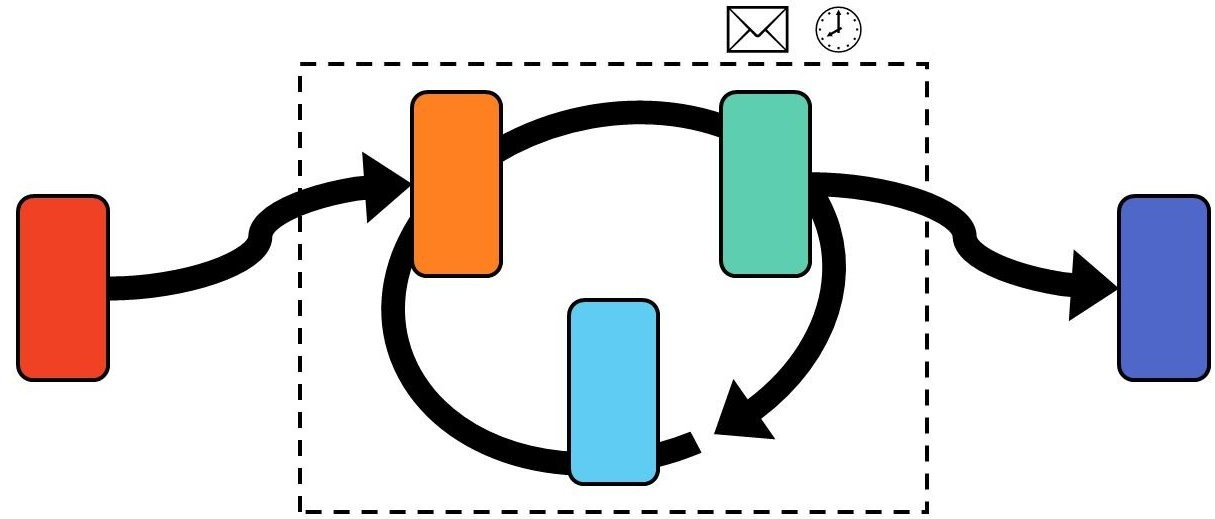
\includegraphics[align=c,width=\linewidth]{img/naiad.jpg}
    Timely Dataflow & 2013~\cite{Naiad2013}
        & 2021~\cite{Timely} & \GreenYes{} & -- \\
    \makecell{
\includegraphics[align=c,width=0.8\linewidth]{img/heron.png} \\ \cite{Heron,kulkarni2015twitter-heron}}
        & 2015 & 2021 & \GreenYes{} & 41 \\
\end{Tabular}

\vspace{1cm}

\caption{A selection of major distributed stream processing systems.}
\label{fig:dsps-examples}
\end{table}
